\chapter{Interfaces gráficas}

A construção de interfaces gráficas se baseia no uso de componentes, que são objetos com capacidade de interagir com o usuário. O Java fornece bibliotecas de componentes para auxiliar na construção de interfaces gráficas. As bibliotecas mais conhecidas são o AWT (Abstract Window Toolkit) e o SWING. Este último é mais atual e possui mais componentes e recursos, mas ainda permite a utilização em conjunto com o anterior. Estas bibliotecas são disponibilizadas através dos pacotes \texttt{java.awt.*} e \texttt{javax.swing.*}.

Algumas IDEs possuem ferramentas para suporte à construção de interfaces gráficas, as quais permitem ao desenvolvedor construí-la de forma visual, arrastando seus componentes e implementando suas ações. Entre as IDEs mais conhecidas com suporte à construção de interfaces gráficas estão o NetBeans e o Eclipse. Este capítulo apresenta uma introdução ao desenvolvimento de aplicações gráficas usando o NetBeans. Desenvolveremos um sistema para cadastro de veículos (\texttt{CadastroVeiculo}).

\section{Construção usando o NetBeans}
O primeiro passo é criar um projeto do tipo \texttt{Aplicação Java} (\texttt{Java Application}). No pacote de códigos-fonte, clique com o botão direito e selecione as opções \texttt{Novo} > \texttt{Form JFrame}. Caso esta opção não seja apresentada, busque-a em \texttt{Outros}. Estes passos criarão uma classe que estende \code{JFrame}, que consiste em uma tela. Portanto, podemos chamar nossa primeira tela (classe) de \code{TelaPrincipal}. A Figura~\ref{fig:gui-criacao-tela} ilustra o processo de criação da primeira tela do sistema.

\begin{figure}[h]
	\centering
	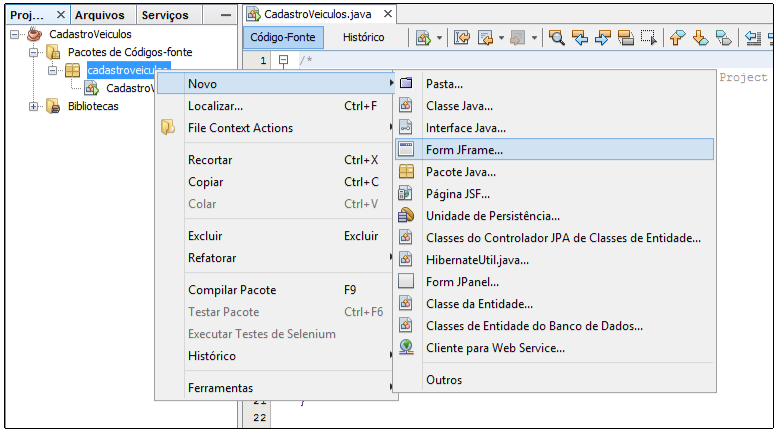
\includegraphics[width=0.6\textheight]{img/gui-criacao-tela}
	\caption{Criação de uma tela (\texttt{JFrame})}
	\label{fig:gui-criacao-tela}
\end{figure}

O NetBeans fornece uma série de ferramentas para suporte à construção de interfaces gráficas. A Figura~\ref{fig:gui-netbeans} mostra a IDE e suas ferramentas. No lado esquerdo, podemos acessar a estrutura do projeto e seus arquivos. Na parte central observamos a tela que está sendo construída. Nela podemos inserir componentes, posicioná-los e configurá-los. Na parte direita (acima) encontramos a paleta de componentes. Através dela é possível selecionar os componentes desejados e arrastá-los até a área de construção da interface. Logo abaixo observa-se as propriedades dos elementos. Basta selecionar um componente inserido na interface e suas propriedades são apresentadas, possibilitando a alteração e ajuste dos seus valores.

\begin{figure}[h]
	\centering
	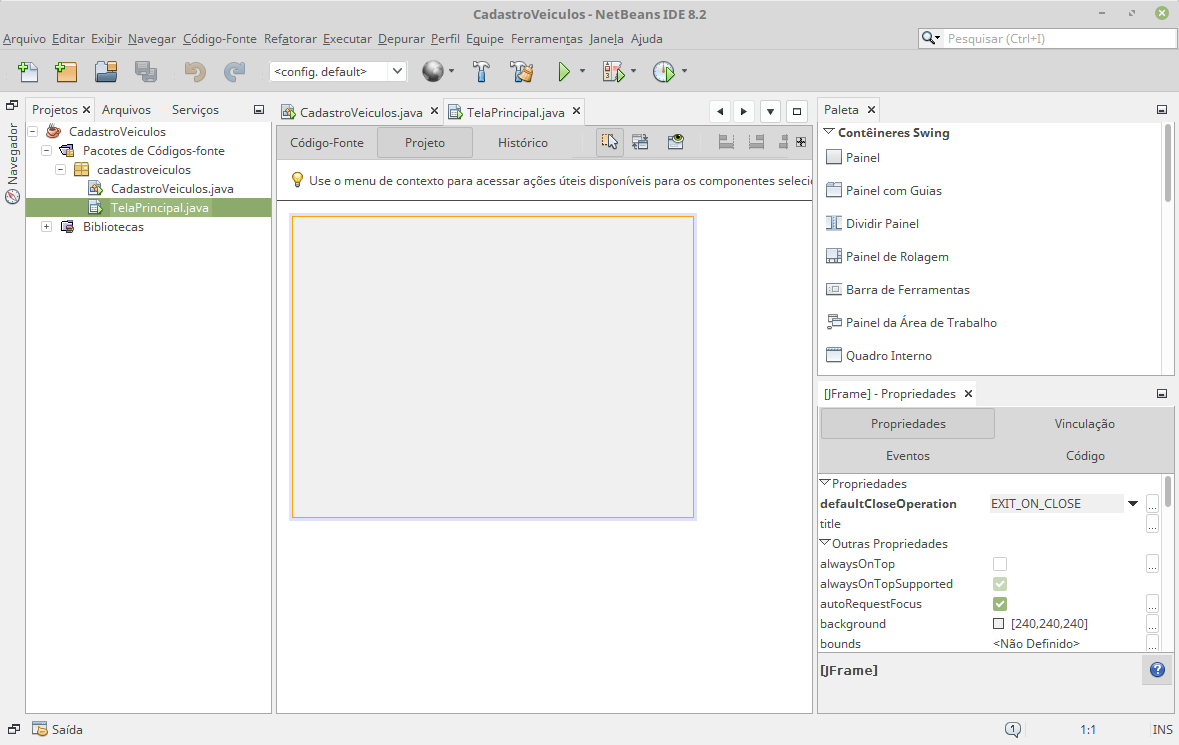
\includegraphics[width=0.6\textheight]{img/gui-netbeans}
	\caption{NetBeans com ferramentas para interfaces gráficas}
	\label{fig:gui-netbeans}
\end{figure}

O componente \texttt{JFrame}, que consiste em uma tela através do qual o usuário interage com o sistema, é criado automaticamente com um método \code{main}, permitindo que a aplicação inicie por ele. O ideal é que uma classe de controle seja responsável por iniciar o sistema e criar as suas telas. Porém, por questões de simplicidade, utilizaremos a \code{TelaPrincipal} como ponto de partida da aplicação. Logo, a classe principal criada no projeto pode ser excluída. A Figura~\ref{fig:gui-estrutura-inicial} mostra a estrutura atual do projeto.

\begin{figure}[h]
	\centering
	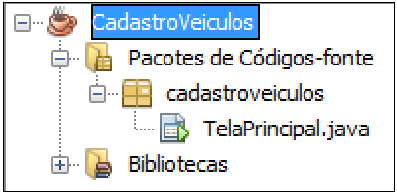
\includegraphics[width=0.4\textheight]{img/gui-estrutura-inicial}
	\caption{Estrutura inicial do projeto}
	\label{fig:gui-estrutura-inicial}
\end{figure}

Logo acima da pré-visualização da interface encontram-se algumas abas (chamadas visões), entre elas \texttt{Código-fonte} e \texttt{Projeto}. Ao selecionar a aba \texttt{Projeto}, as ferramentas de construção visuais são apresentadas. Ao selecionar a aba \texttt{Código-fonte}, o código gerado é apresentado e o programador pode fazer as alterações desejadas e a implementação dos métodos da aplicação.

Abaixo é apresentado o código para a tela inicial criada. Perceba que a classe estende \code{JFrame}. O método \code{main} cria a janela e a torna visível. No construtor, todos os componentes inseridos na tela são inicializados. Nesta classe podemos definir nossas variáveis, como a lista de veículos e os objetos necessários à sua manipulação.

\begin{minted}{java}
public class TelaPrincipal extends javax.swing.JFrame {
	
	public TelaPrincipal() {
		initComponents();
	}
	
	@SuppressWarnings("unchecked") 
	//Generated code
	
	public static void main(String args[]) { 
		java.awt.EventQueue.invokeLater(new Runnable() {
			public void run() { 
				new TelaPrincipal().setVisible(true); 
			}
		});
	}
}    
\end{minted}
    
\section{Barra de menu, eventos e ações}

Utilizando a visão de \texttt{Projeto}, na categoria \texttt{Menus Swing} da paleta de componentes, arraste o elemento \texttt{Barra de Menu} para a janela. Será criado um menu com as opções \texttt{File} e \texttt{Edit}. Clicando com o botão direito sobre estes itens é possível:

\begin{itemize}
	\item Editar o texto que é apresentado em tela.
	\item Alterar o nome da variável (objeto) do componente.
	\item Adicionar itens a esta opção do menu (\texttt{Adicionar da Paleta} > \texttt{Item de Menu}).
	\item Para cada item adicionado, é possível realizar as mesmas ações.
\end{itemize}

Com o uso destas opções, crie configuração do menu apresentada na Figura~\ref{fig:gui-menu}.

\begin{figure}[h]
	\centering
	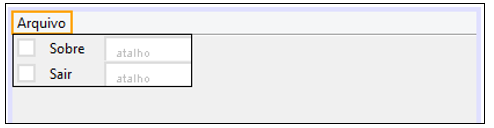
\includegraphics[width=0.4\textheight]{img/gui-menu}
	\caption{Menu para a aplicação \texttt{CadastroVeiculos}}
	\label{fig:gui-menu}
\end{figure}

\textbf{OBS:} é importante definirmos nomes sugestivos a cada objeto que será manipulado, de forma a dar legibilidade ao código. Exemplos: \code{menuArquivo}, \code{menuSobre} e \code{menuSair}.

Execute a aplicação e veja o resultado, que deve ser parecido com o apresentado na Figura~\ref{fig:gui-aplicacao-inicial}. O título da tela (``Cadastro de Veículos'') pode ser definido na propriedade \texttt{title} da janela. Selecionando a janela, suas propriedades são apresentadas na parte direita da interface. Basta, portanto, localizar e alterar a propriedade desejada.

\begin{figure}[h]
	\centering
	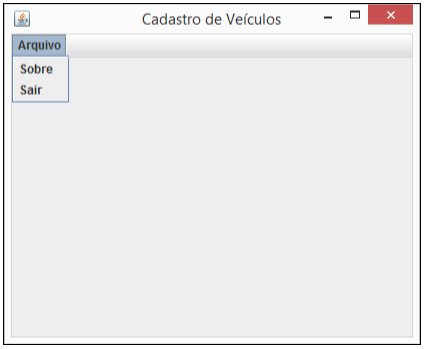
\includegraphics[width=0.4\textheight]{img/gui-aplicacao-inicial}
	\caption{Aplicação inicial com barra de menu}
	\label{fig:gui-aplicacao-inicial}
\end{figure}

do o usuário clicar na opção \texttt{Sobre}, devemos apresentar uma janela com as informações de desenvolvimento da aplicação. Podemos apresentar uma caixa de diálogo (\texttt{JOptionPane}). Logo, basta definirmos a exibição da janela no evento de ação do item de menu correspondente. Ou seja, quando o usuário clica no item, o método (chamado evento) é disparado.

Para isso, clique com o botão direito no item \texttt{Sobre} e selecione as opções \texttt{Eventos} > \texttt{Action} > \texttt{actionPerformed}. A Figura~\ref{fig:gui-action-performed} mostra estas ações. Com isso, o NetBeans criará um método que é invocado sempre que o item de menu for selecionado pelo usuário. Nele, podemos implementar o comportamento desejado.

\begin{figure}[h]
	\centering
	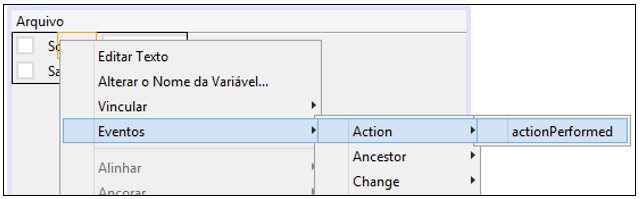
\includegraphics[width=0.4\textheight]{img/gui-action-performed}
	\caption{Definição do evento \texttt{actionPerformed}}
	\label{fig:gui-action-performed}
\end{figure}

O trecho de código abaixo mostra a implementação do método que é disparado no evento de ação do componente \code{menuSobre}. Quando o usuário clicar neste item, será apresentado uma caixa de diálogo com informações do desenvolvimento. Repare que, uma vez que temos uma janela no sistema, podemos defini-la como componente pai da caixa de diálogo. Isso é feito no primeiro argumento do método \code{showMessageDialog}. A Figura~\ref{fig:gui-tela-sobre} mostra o resultado da execução do evento de clique no item de menu \texttt{Sobre}.

\begin{minted}{java}
private void menuSobreActionPerformed(java.awt.event.ActionEvent evt) {
	JOptionPane.showMessageDialog(this,
		"Desenvolvido na disciplina de Programação I - 25PRO1\n"
		+ "Universidade do Estado de Santa Catarina\n"
		+ "Centro de Educação Superior do Alto Vale do Itajaí");
}
\end{minted}

\begin{figure}[h]
	\centering
	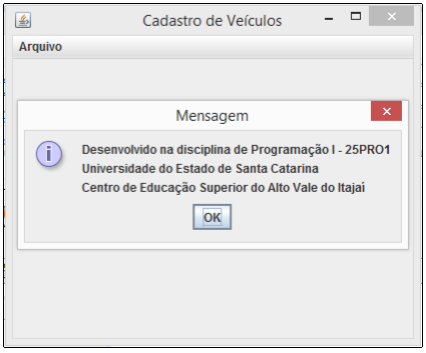
\includegraphics[width=0.4\textheight]{img/gui-tela-sobre}
	\caption{Execução da ação do menu \texttt{Sobre}}
	\label{fig:gui-tela-sobre}
\end{figure}

Faremos o mesmo procedimento para definir o código a ser executado quando o usuário clicar no item \texttt{Sair}. Neste caso, a tarefa é fechar a janela e finalizar a aplicação, mostrando uma mensagem de encerramento. A finalização da aplicação é obtida pelo método \code{dispose}. O trecho de código abaixo mostra sua implementação, enquanto a Figura~\ref{fig:gui-tela-sair} mostra o resultado da sua execução.

\begin{minted}{java}
private void menuSairActionPerformed(java.awt.event.ActionEvent evt) {
	JOptionPane.showMessageDialog(this, "Encerrando a aplicação...");
	dispose();
}
\end{minted}

\begin{figure}[h]
	\centering
	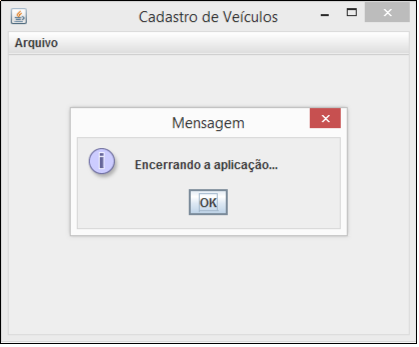
\includegraphics[width=0.4\textheight]{img/gui-tela-sair}
	\caption{Execução da ação do menu \texttt{Sair}}
	\label{fig:tela-sair}
\end{figure}

\section{Entidade Veiculo}

Como a aplicação tem como objetivo o cadastro de veículos, precisamos definir a entidade \code{Veiculo}. Esta classe possui modelo, marca e ano, bem como seus métodos construtores e acessores. A Figura~\ref{fig:gui-veiculo} mostra sua representação UML e o código correspondente é apresentado na sequência.

\begin{figure}[h]
	\centering
	
	\begin{tikzpicture}
	\umlclass{Veiculo}{
		-- modelo: String \\
		-- marca: String \\
		-- ano: int
	}{
		+ métodos construtores \\
		+ métodos acessores
	}	
	\end{tikzpicture}
	
	\caption{Representação UML da classe \code{Veiculo}}
	\label{fig:gui-veiculo}
\end{figure}

\begin{minted}{java}
public class Veiculo {
	private String modelo;
	private String marca;
	private int ano;
	
	//Métodos construtores e acessores
}
\end{minted}


\section{Componentes da tela}

A tela principal deve apresentar um formulário através do qual o usuário poderá cadastrar, consultar, alterar e excluir veículos. Os componentes disponíveis na paleta (alguns deles) são apresentados pela Figura~\ref{fig:gui-paleta}. Para construir a interface desejada, utilizaremos os componentes listados abaixo (entre parêntesis é apresentada a classe que implementa cada componente).

\begin{itemize}
	\item \texttt{Label} (\code{JLabel}): rótulo ou saída de texto na tela.
	\item \texttt{TextField} (\code{JTextField}): campo de entrada de texto.
	\item \texttt{Button} (\code{JButton}): botão de ação.
\end{itemize}

\begin{figure}[h]
	\centering
	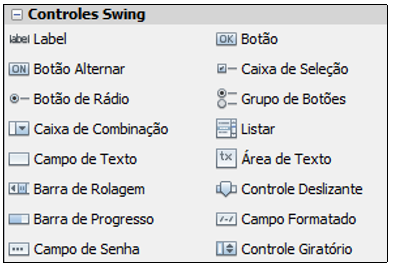
\includegraphics[width=0.4\textheight]{img/gui-paleta}
	\caption{Paleta de componentes \texttt{Swing}}
	\label{fig:gui-paleta}
\end{figure}

A Figura~\ref{fig:gui-formulario} apresenta o formulário formado pelos componentes supracitados. Do lado esquerdo podemos observar os elementos \texttt{Label}, que formam os textos \texttt{Modelo.:}, \texttt{Marca.:} e \texttt{Ano.:}. Os campos de entrada de texto são componentes \texttt{TextField} e os botões são componentes \texttt{Button}. Assim como nos itens de menu, estes objetos devem receber um nome sugestivo e seu texto de apresentação deve ser definido nas propriedades. Posicione cada elemento e define os textos de exibição e nomes sugestivos aos objetos, seguindo a proposta da Figura~\ref{fig:gui-formulario}.

\begin{figure}[h]
	\centering
	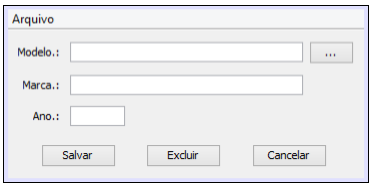
\includegraphics[width=0.4\textheight]{img/gui-formulario}
	\caption{Formulário da tela principal}
	\label{fig:gui-formulario}
\end{figure}

\section{Funcionalidades}

Para implementar as funcionalidades, a classe \code{TelaPrincipal} deverá manter uma lista de veículos (onde os registros serão armazenados) e um objeto da classe \code{Veiculo} (que representará o registro manipulado pelo usuário).

\begin{minted}{java}
public class TelaPrincipal extends javax.swing.JFrame {

	private List<Veiculo> listaVeiculos = new ArrayList<Veiculo>();
	private Veiculo veiculo = new Veiculo();

	//...
}
\end{minted}

\subsection{Salvar registro}
Da mesma forma como é feito com os menus, é possível definir métodos que serão executados quando os botões forem clicados. O processo é o mesmo, definindo um evento do tipo \texttt{actionPerformed}.

O botão \texttt{Salvar} serve para gravar um novo registro na lista, com base nas informações digitadas pelo usuário, ou gravar as alterações feitas pelo usuário em um objeto previamente recuperado da lista. Logo, os passos que devem ser implementados são:

\begin{itemize}
	\item Recuperar os valores digitados pelo usuário no formulário.
	\item Atualizar os atributos do objeto veiculo com os valores recuperados.
	\item Se o objeto não se encontra na lista, é um novo registro e deve ser incluído na mesma. Caso contrário, trata-se de uma alteração e a atualização do objeto já é suficiente.
	\item Instanciar um novo objeto em veiculo, permitindo o cadastro de um novo registro.
	\item Limpar os campos do formulário para que o usuário possa cadastrar um novo registro.
\end{itemize}

O trecho de código abaixo mostra a implementação resultante do método de salvar. Repare que isto é feito no evento de ação do componente \code{btSalvar}. As linhas 2 a 4 recuperam os valores informados pelo usuário na tela. Perceba que é possível acessar os objetos dos componentes, recuperando o valor digitado através do método \code{getText}. As linhas 6 a 8 setam os valores recuperados aos atributos do objeto \code{veiculo}. Nas linhas 10 a 12, se o objeto não se encontra na lista, trata-se de um novo registro e ele deve ser inserido na mesma. Caso contrário, trata-se de uma alteração de um registro existente (pois já encontra-se na lista) e a atualização do objeto já é suficiente. A linha 13 instancia um novo objeto para permitir o cadastro de um novo registro. Finalmente, as linhas 15 a 17 limpam os campos da tela após o cadastro ou alteração.

\begin{minted}{java}
private void btSalvarActionPerformed(java.awt.event.ActionEvent evt) {
	String modelo = edModelo.getText();
	String marca = edMarca.getText();
	int ano = Integer.parseInt(edAno.getText());
	
	veiculo.setModelo(modelo);
	veiculo.setMarca(marca);
	veiculo.setAno(ano);
	
	if(!listaVeiculos.contains(veiculo)) {
		listaVeiculos.add(veiculo);
	}
	veiculo = new Veiculo();
	
	edModelo.setText("");
	edMarca.setText("");
	edAno.setText("");
}
\end{minted}

\subsection{Cancelar preenchimento}

O botão \texttt{Cancelar} deve limpar todos os campos. Caso os valores nos campos sejam referentes a um objeto pesquisado pelo usuário, a referência armazenada em \code{veiculo} deve ser removida e uma nova instância atribuída ao objeto. Isso é feito no método apresentado abaixo, vinculado ao botão \code{btCancelar}.

\begin{minted}{java}
private void btCancelarActionPerformed(java.awt.event.ActionEvent evt) {
	edModelo.setText("");
	edMarca.setText("");
	edAno.setText("");
	veiculo = new Veiculo();
}
\end{minted}

\subsection{Excluir registro}

O botão \texttt{Excluir} remove da lista de veículos um registro pesquisado anteriormente. Como o registro pesquisado se encontra armazenado no objeto \code{veiculo}, basta removê-lo da lista, atribuir uma nova instância a ele e limpar os campos da tela. Isso é feito no método apresentado abaixo, vinculado ao botão \code{btExcluir}.

\begin{minted}{java}
private void btExcluirActionPerformed(java.awt.event.ActionEvent evt) {
	listaVeiculos.remove(veiculo);
	this.veiculo = new Veiculo();

	edModelo.setText("");
	edMarca.setText("");
	edAno.setText("");
}
\end{minted}

\subsection{Pesquisar registro}

O botão \texttt{Pesquisar} permite recuperar um objeto da lista de veículos e preencher os campos do formulário com os valores dos seus atributos. Essa pesquisa é feita com base no valor de modelo informado pelo usuário, por isso o botão se localiza ao lado deste campo.

Caso o veículo seja encontrado, sua referência deve ser armazenada no objeto \code{veiculo} e os campos do formulário são preenchidos com os valores dos seus atributos. Com isso, caso o usuário modifique os valores dos campos e clique em \texttt{Salvar}, o objeto da lista de veículos será atualizado, ao invés de incluído um novo objeto. Caso o usuário clique em \texttt{Excluir}, o objeto será removido da lista. Caso o usuário clique em \texttt{Cancelar}, nada é realizado e os campos e o objeto são ``reiniciados''.

O código vinculado ao evento de ação do botão \texttt{Pesquisar} é apresentado abaixo. Na linha 2, o modelo digitado pelo usuário é recuperado. A lista de veículos é percorrida e, caso encontrado um objeto com o modelo buscado, sua referência é armazenada em \code{veiculo} e seus atributos são inseridos nos campos do formulário (linhas 4 a 11).

\begin{minted}{java}
private void btPesquisarActionPerformed(java.awt.event.ActionEvent evt) {
	String modelo = edModelo.getText();

	for(Veiculo v : listaVeiculos) {
		if(v.getModelo().equals(modelo)) {
			veiculo = v;
			edModelo.setText(veiculo.getModelo());
			edMarca.setText(veiculo.getMarca());
			edAno.setText(String.valueOf(veiculo.getAno()));
			break;
		}
	}
}
\end{minted}

\subsection{Excluir registro}

Uma característica importante do botão \texttt{Excluir} é o fato de ele não fazer sentido quando o usuário está cadastrando um novo veículo. Sua funcionalidade só pode ser executada quando o usuário carregar um veículo previamente cadastrado. Para evitar problemas, podemos desabilitar o botão quando o mesmo não deve ser clicado, impedindo que o usuário execute o método vinculado a ele e deixando claro sua impossibilidade de uso.

Isso pode ser feito feito modificando a propriedade \texttt{enabled} através do método \code{setEnabled(true)} ou \code{setEnabled(false)}, habilitando e desabilitando o componente. O trecho de código abaixo apresenta um exemplo do uso deste método.

\begin{minted}{java}
btExcluir.setEnabled(true);
btExcluir.setEnabled(false);
\end{minted}

O botão \texttt{Excluir} deve ser habilitado nos seguintes casos:

\begin{itemize}
	\item Quando a ação de pesquisa encontra o objeto e o carrega na tela, permitindo ao usuário excluir o veículo, se desejado.
\end{itemize}

O botão \texttt{Excluir} deve ser desabilitado nos seguintes casos:

\begin{itemize}
	\item Quando a ação de salvar é realizada, pois pode se tratar de um objeto carregado da lista, com suas alterações sendo salvas.
	\item Quando a ação de cancelar é realizada, pois pode se tratar de um objeto carregado da lista, onde o usuário está cancelando sua alteração.
	\item Quando a ação de exclusão é realizada, pois ao concluir a exclusão de um registro, uma nova instância é definida e não é possível excluir novamente.
	\item Quando a aplicação inicia, pois o botão deve estar desabilitado por padrão. Isso pode ser feito no construtor da classe, após a inicialização dos seus componentes (trecho de código abaixo).
\end{itemize}

\begin{minted}{java}
public TelaPrincipal() {
	initComponents();
	btExcluir.setEnabled(false);
}
\end{minted}

\section{Outros componentes}

Existem muitos outros componentes swing para a construção de interfaces gráficas interativas. A Figura~\ref{fig:gui-outros-componentes} apresenta a aplicação de componentes de \textit{checkbox}, \textit{radio button}, menu de seleção, campo de senha, área de texto e caixa de seleção.

\begin{figure}[h]
	\centering
	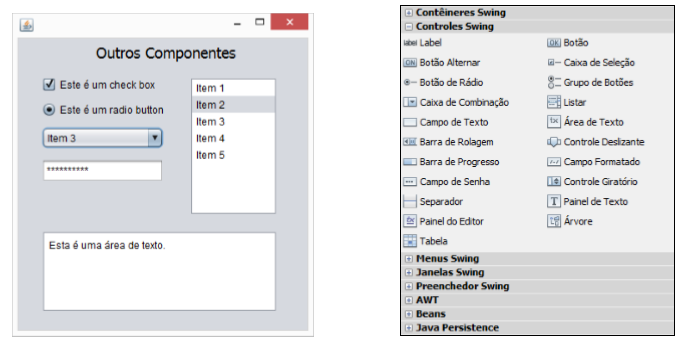
\includegraphics[width=0.4\textheight]{img/gui-outros-componentes}
	\caption{Outros componentes \texttt{swing}}
	\label{fig:gui-outros-componentes}
\end{figure}

Para consultar a documentação dos componentes que deseja utilizar, consulte \url{http://docs.oracle.com/javase/8/docs/api}.